\documentclass[letter,12pt]{article}
\usepackage{amsmath}
\usepackage{graphicx}
\usepackage{glosstex}
\usepackage[utf8]{inputenc}
\usepackage[spanish]{babel}
\usepackage{tikz,stackengine}

%opening
\title{Reporte 01 Evaluación 29 10 2019}
\author{Eduardo Alexis Valencia Dorantes}
\date{30/Octubre/2019}
\begin{document}
	
\maketitle{Compilación de RaízCuadrada.tex}

\begin{abstract}
Se presentara el procedimiento que se seguirá para compilar el archivo que envió el profesor Luis Enrique Serrano Gómez
\end{abstract}

\section*{Descargar el documento}
1. Se abre el Classroom de la clase de "Taller de Herramientas Computacionales 2020-1", dentro se da clic en la tarea "Evaluación 29 10 2019,sección práctica."

\begin{figure}[h]
	\centering
	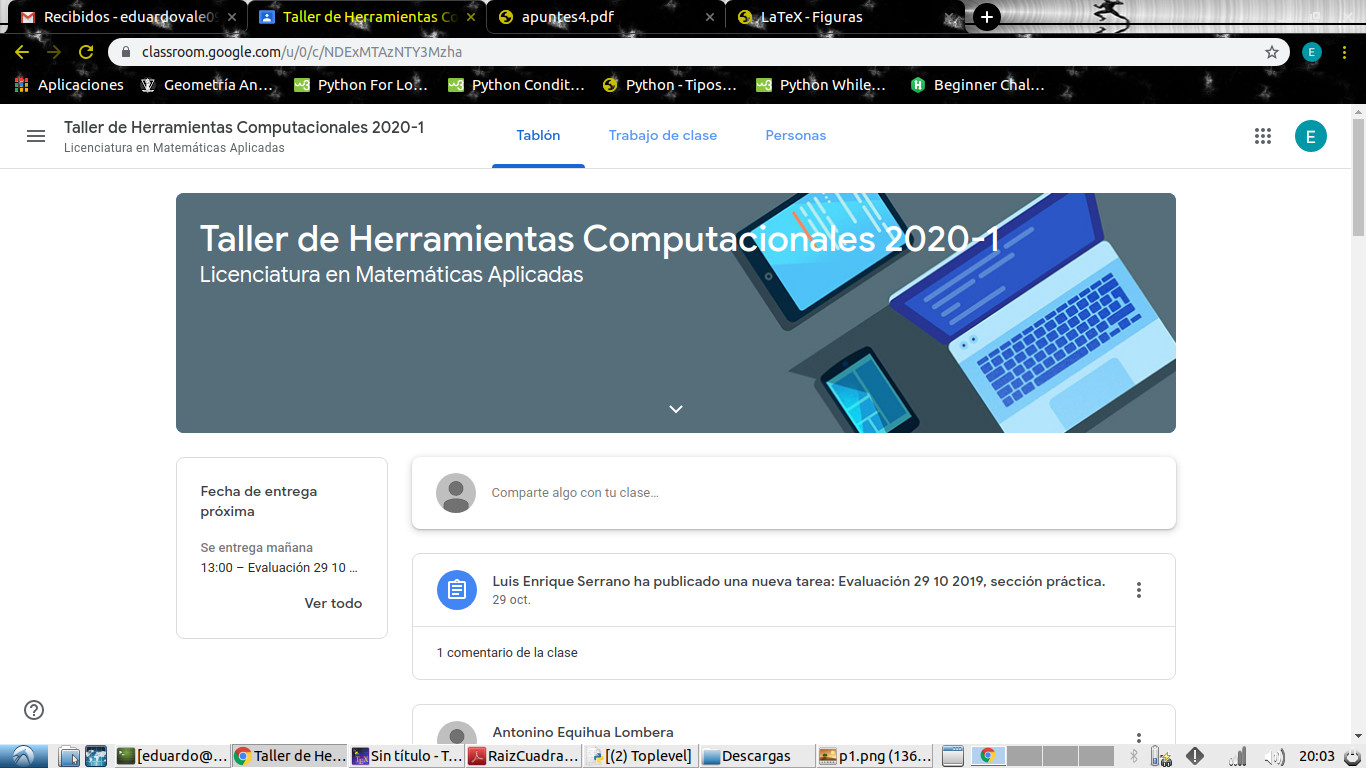
\includegraphics[width=0.8\linewidth]{../Imagenes/p2.jpg}
	\caption{}
	\label{fig:p2}
\end{figure}

\newpage
2. Dentro de esta tarea se buscara el archivo adjunto con el nombre de "RaízCuadrada.py" y se selecciona.

\begin{figure}[h]
	\centering
	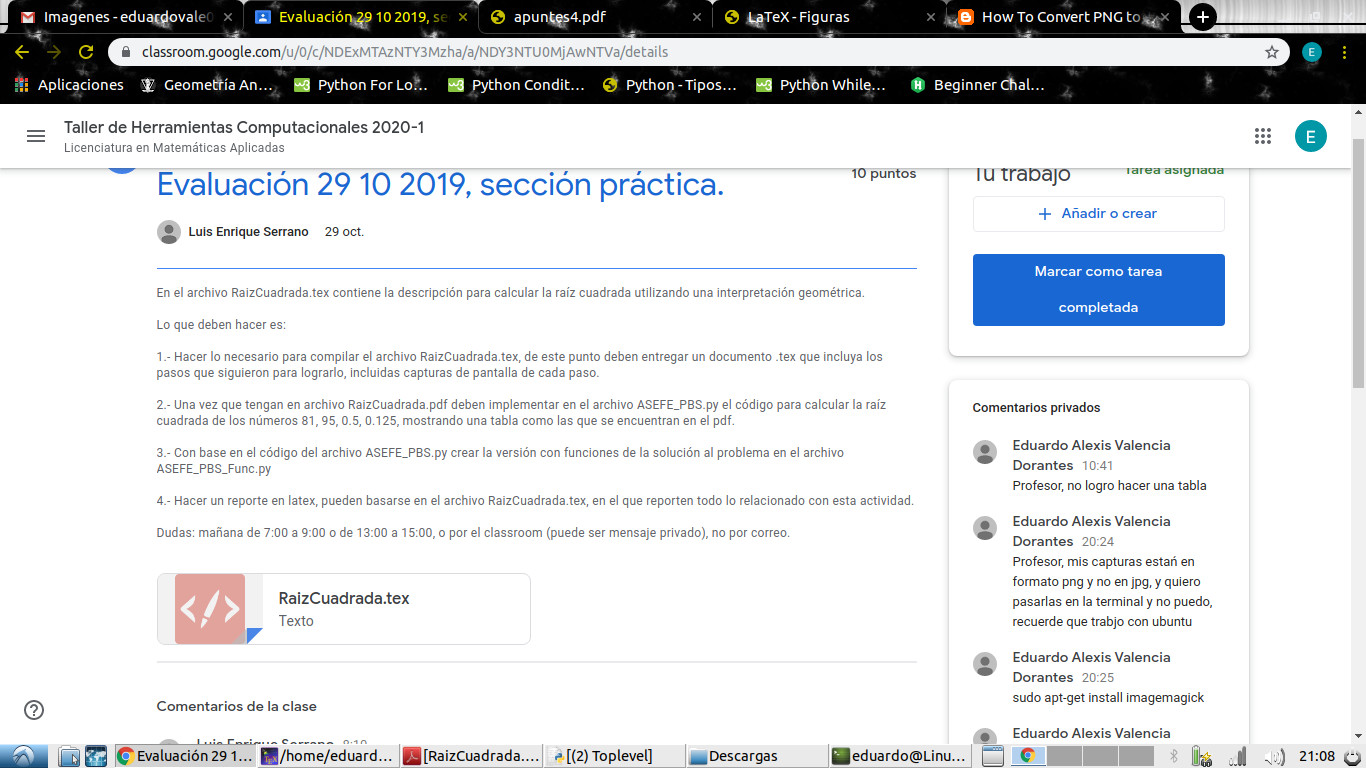
\includegraphics[width=0.7\linewidth]{../../Imagenes/p3.jpg}
	\caption{}
	\label{fig:p3}
\end{figure}


3. Dentro de está página se buscará la opción de descargar y se seleccionará.

\begin{figure}[h]
	\centering
	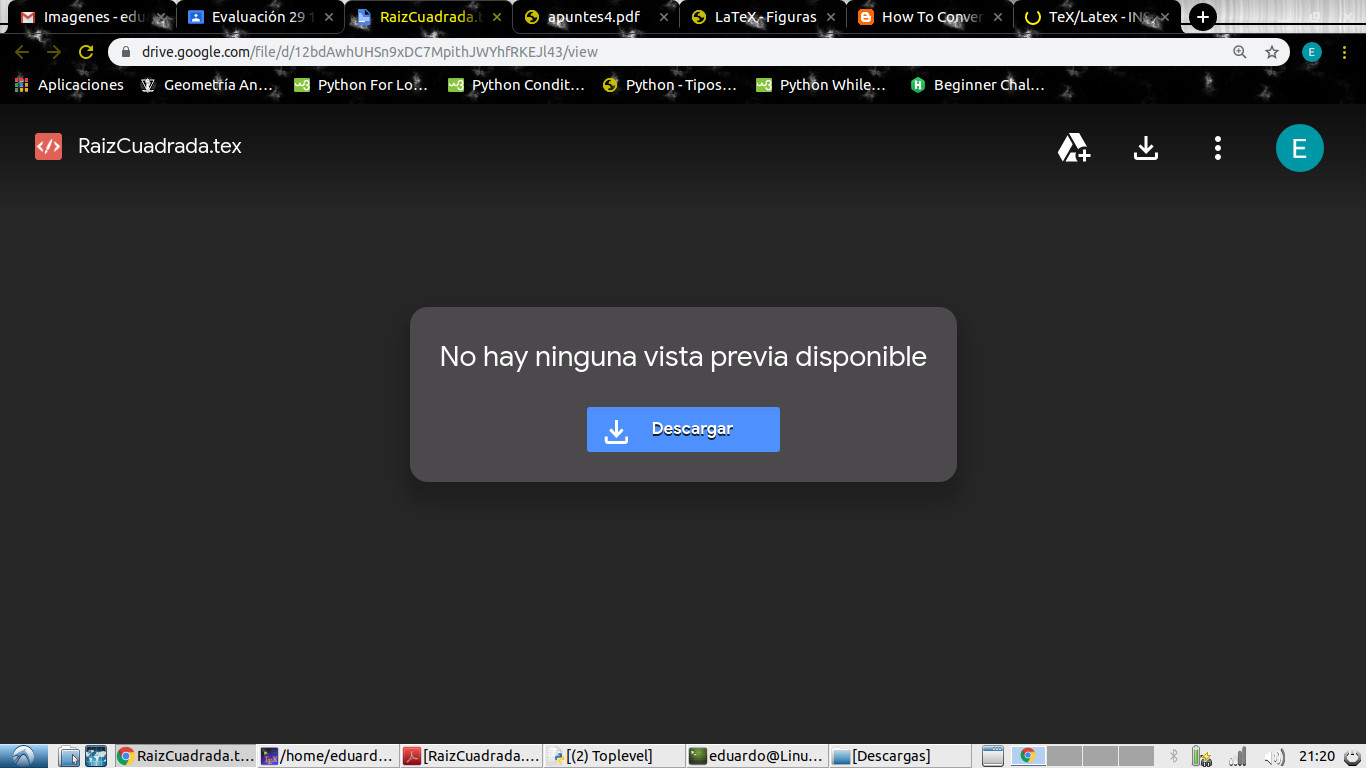
\includegraphics[width=0.8\linewidth]{../../Imagenes/p4.jpg}
	\caption{}
	\label{fig:p4}
\end{figure}
\newpage
\section*{Se abrirá el documento}
4. Se abrirá el gestor de archivos y dentro de este se buscará el archivo descargado con la leyenda "RaízCuadrada.tex" y se seleccionara.

\begin{figure}[h]
	\centering
	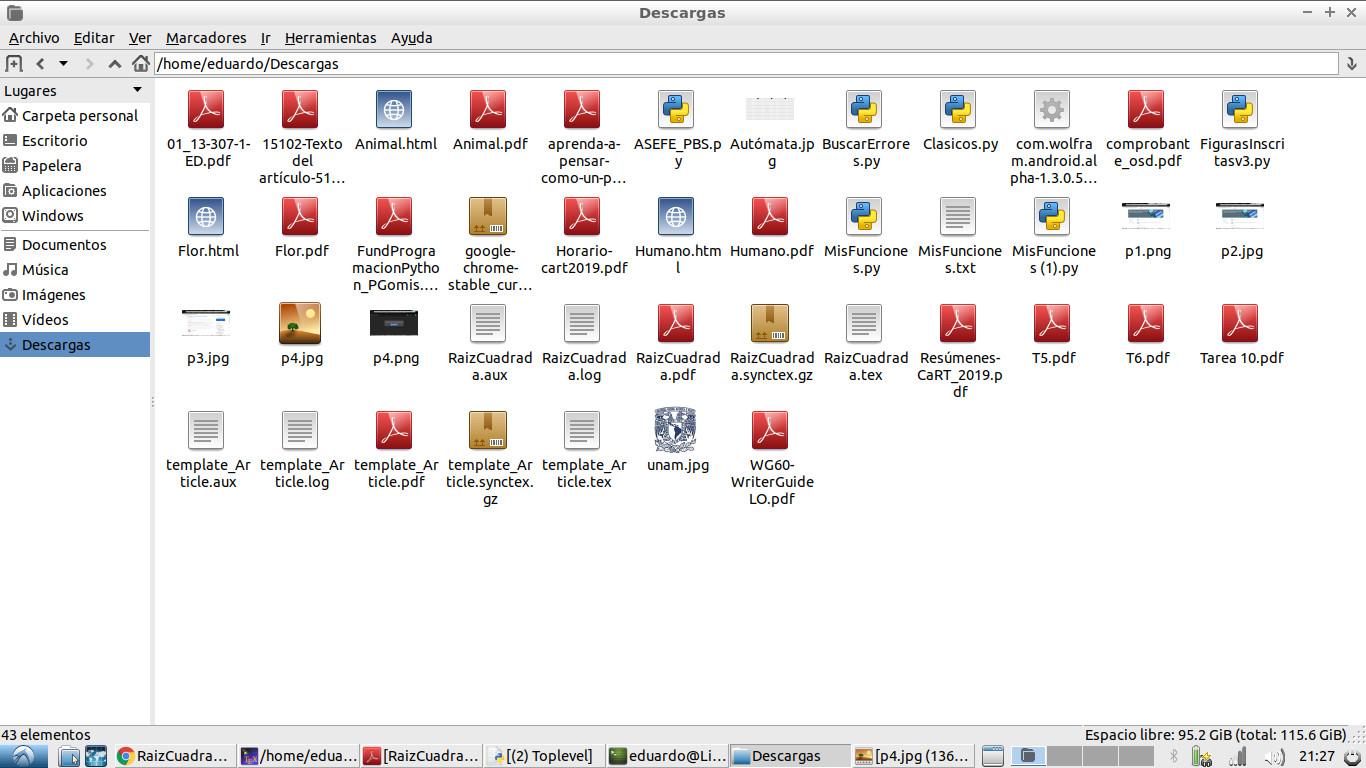
\includegraphics[width=0.8\linewidth]{../../Imagenes/p5.jpg}
	\caption{}
	\label{fig:p5}
\end{figure}

5. Ya abierto el documento de LaTex, al compilar el archivo; este no marca error ya que falta que se instalen dos módulos, una con el nombre de "tikz", y a la otra con el nombre de "stackengine".

Para descargarlas, dado que este caso estamos trabajando con lubuntu, que es otro sistema operativo de Linux, este cuenta con un "Gestor de paquetes Synaptic" el cual se encuentra en las "Herramientas del Sistema".
Para entrar te pedirá tu contraseña y podrás ingresar y se muestra una página de la siguiente manera:

\begin{figure}[h]
	\centering
	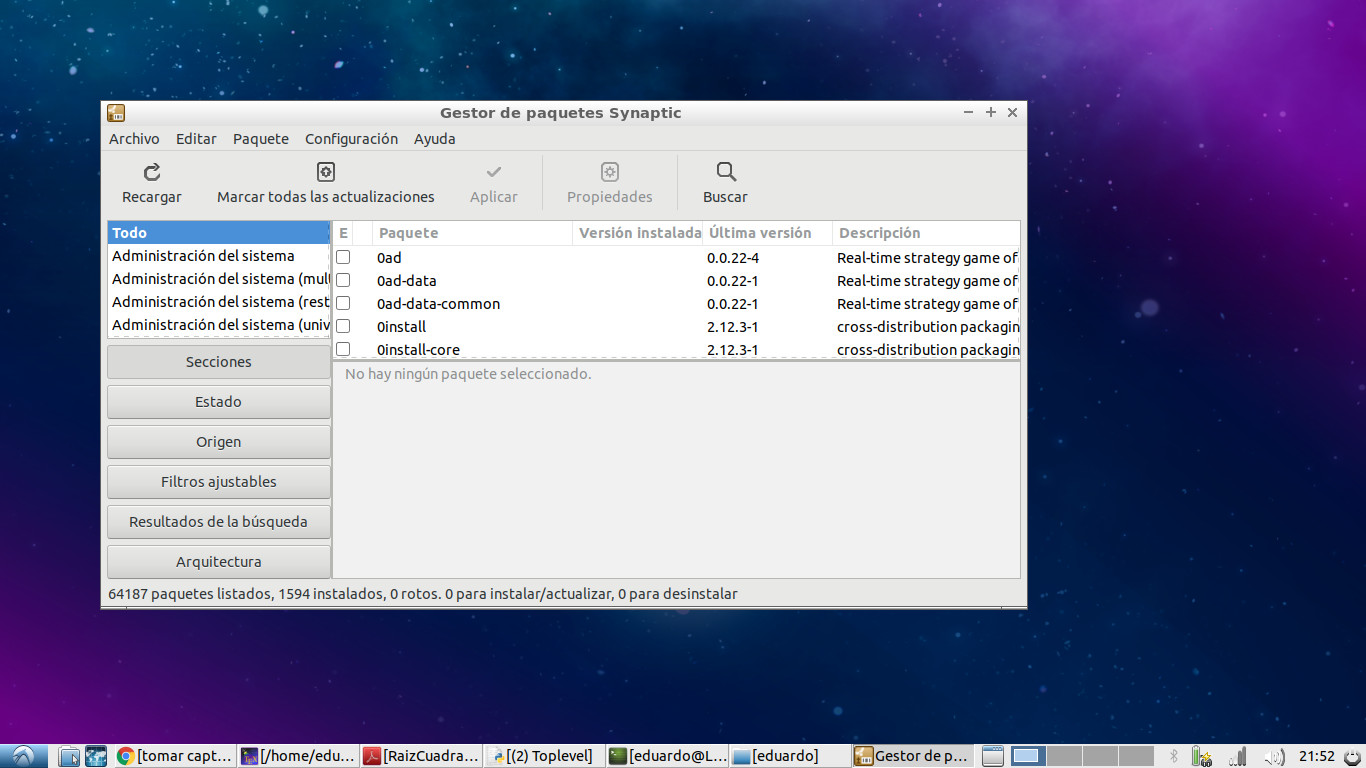
\includegraphics[width=0.8\linewidth]{../../Imagenes/p6.jpg}
	\caption{}
	\label{fig:p6}
\end{figure}
\newpage
6. Se puede encontrar fácilmente la sección que dice "Buscar" en donde escribiremos el nombre de las dos módulos, uno a la vez y presionaremos Enter, haciendo esto nos arrojará una lista con las posibles opciones.
Buscaremos la correspondientes, las seleccionaremos y le daremos aplicar y ya estarán los modulos instalados para poder compilar el programa.

\begin{figure}[h]
	\centering
	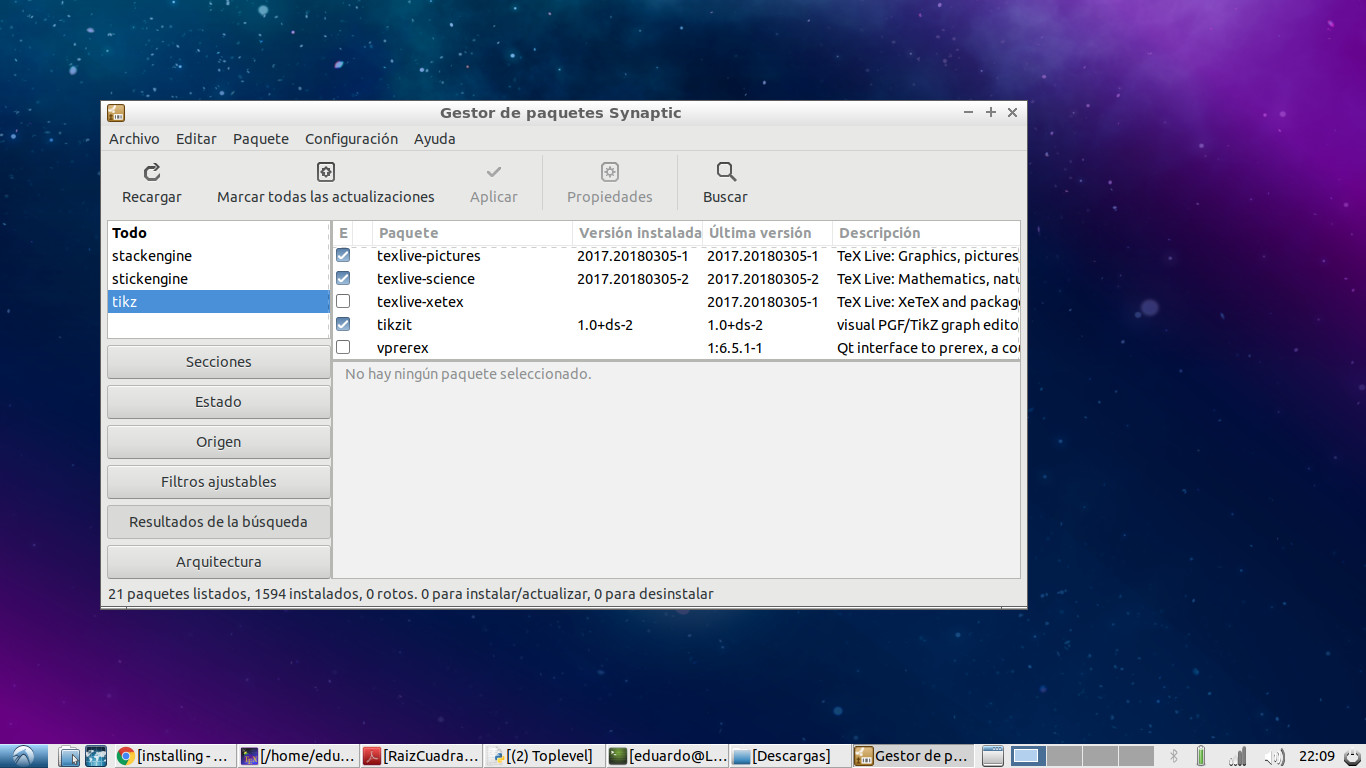
\includegraphics[width=0.8\linewidth]{../../Imagenes/p7.jpg}
	\caption{}
	\label{fig:p7}
\end{figure}

\begin{figure}[h]
	\centering
	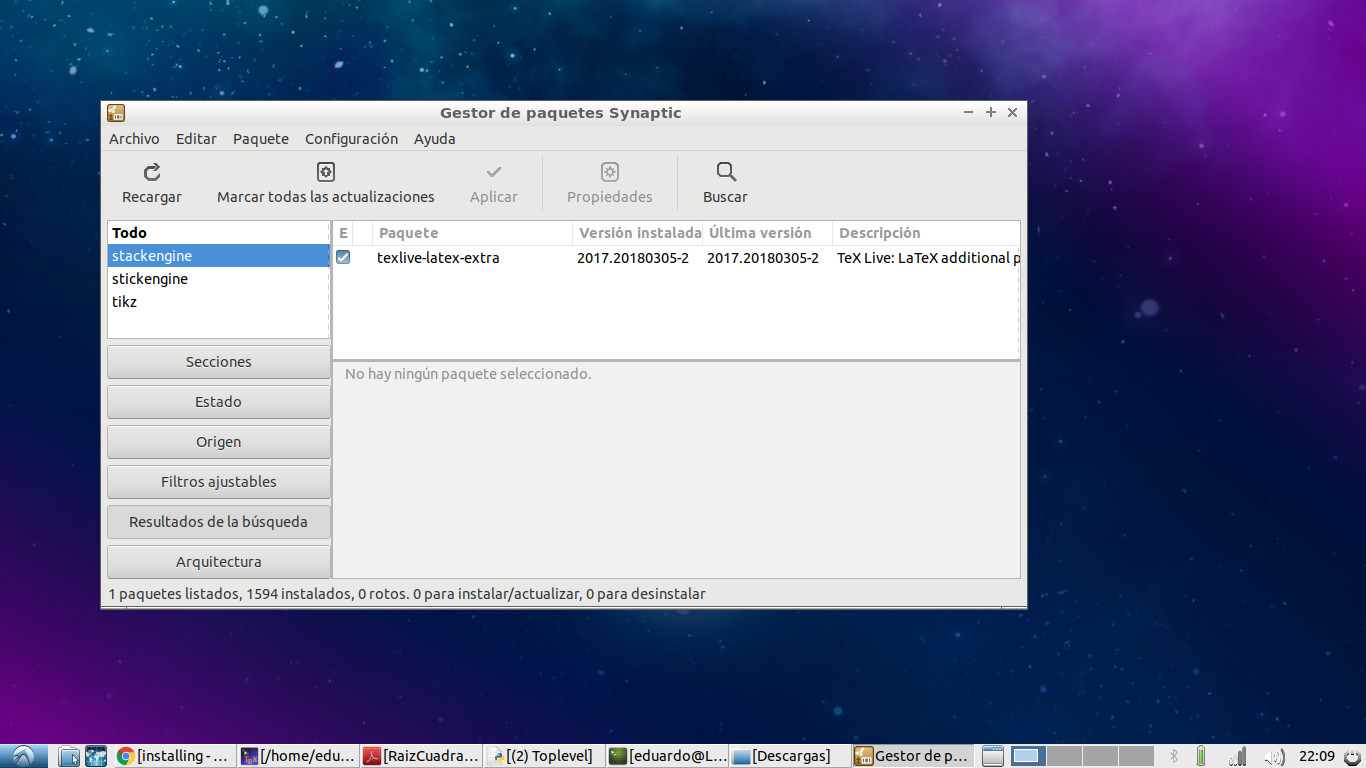
\includegraphics[width=0.8\linewidth]{../../Imagenes/p8.jpg}
	\caption{}
	\label{fig:p8}
\end{figure}
\newpage
\begin{figure}[h]
	\centering
	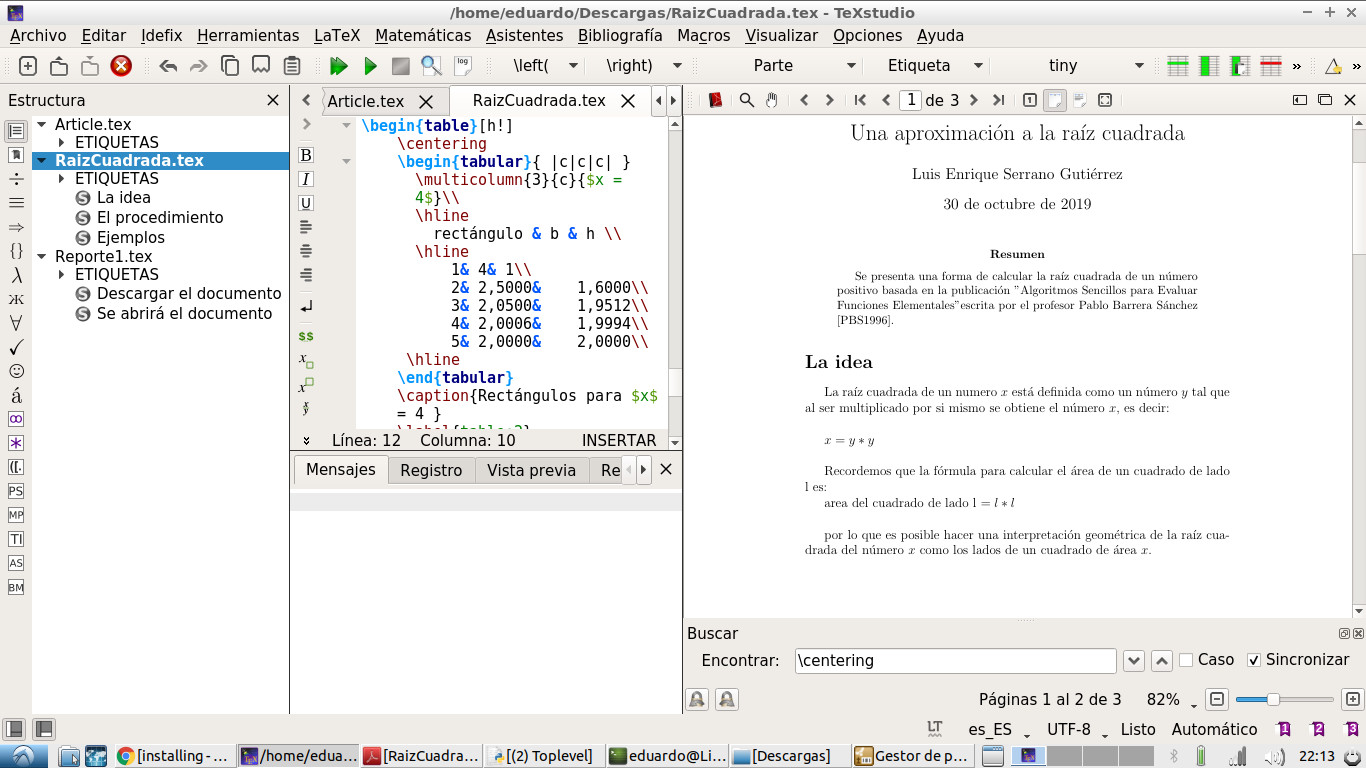
\includegraphics[width=0.8\linewidth]{../../Imagenes/p9.jpg}
	\caption{}
	\label{fig:p9}
\end{figure}
\newpage
\section*{Abrir en PDF}
7. Dentro de nuetra ventana de LaTex hay un recuadro de color rojo que se llama "Visor Externo" que es para ver el archivo en un PDF, se dará clic sobre este icono y nos mandará a una nueva ventana con el archivo en PDF.

\begin{figure}[h]
	\centering
	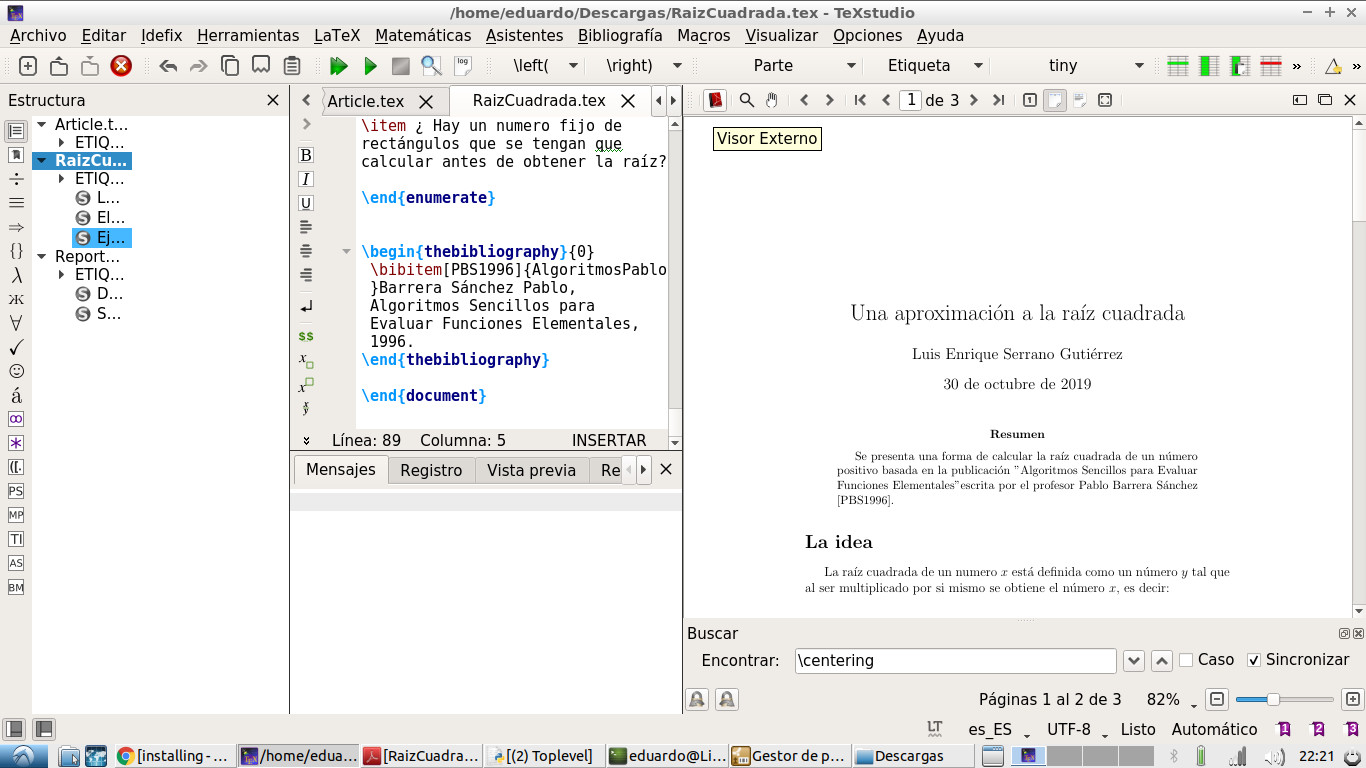
\includegraphics[width=0.8\linewidth]{../../Imagenes/p10.jpg}
	\caption{}
	\label{fig:p10}
\end{figure}

\begin{figure}[h]
	\centering
	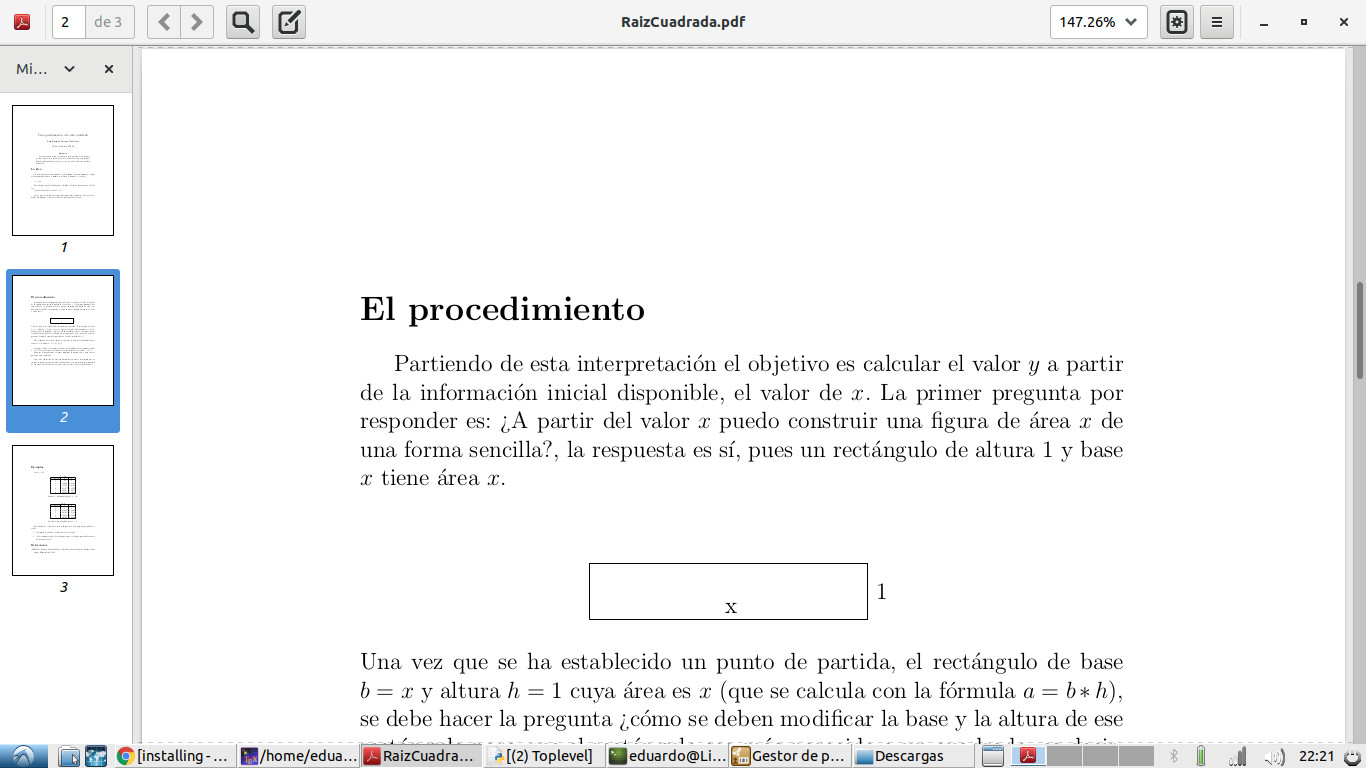
\includegraphics[width=0.8\linewidth]{../../Imagenes/p11.jpg}
	\caption{}
	\label{fig:p11}
\end{figure}
\newpage
8. Este es todo el proceso para abrir el documento "RaízCuadrada.py"


\end{document}

